\documentclass[a4paper]{article}

\usepackage{float}
\usepackage[english]{babel}
\usepackage[utf8]{inputenc}
\usepackage{amsmath}
\usepackage{listings}
\usepackage{graphicx}
\usepackage[colorinlistoftodos]{todonotes}

\definecolor{pblue}{rgb}{0.1,0.1,1}
\definecolor{pgreen}{rgb}{0,0.7,0}
\definecolor{pred}{rgb}{1.0,0,0}
\definecolor{pgrey}{rgb}{0.46,0.45,0.48}


\lstset{
numbers=left,
commentstyle=\color{pgreen},
keywordstyle=\color{pblue},
stringstyle=\color{pred},
xrightmargin=1pt,
breaklines=true,
tabsize=2,
language=java,
basicstyle=\footnotesize
}

\title{Probabilistic Reasoning Over Time}

\author{Jack Foster Terwilliger}

\date{March 8, 2014}

\begin{document}
\maketitle

\section{Introduction}

In partially observable noisy environments, an agent must make decisions despite its incomplete and potentially incorrect knowlege of the state of the environment. In such cases, the agent must infer what is unobservable in the environment from what is observable. In order to make use of its observations for inference, the agent must also have prior knowlege about 1.) its environment: how the environment changes over time and 2.) how observations are emitted by the environment and sensed by the agent. 

In this paper I will explore the use of HMMs and the forward, forwardbackward, and Viterbi algorithms to solve a robot location problem given a partially observable maze. In my code, I used the linear algebra java library, la4j.


\section{Sensor Robot Problem}

In the Sensor Robot Problem, a color sensing robot is placed in a maze with colored tiles and must locate its position in the maze. The robot is given a sequence of observations from its sensors (which are prone to error) and knowlege of the maze. It uses this information as evidence to form a probabilistic distribution over possible locations.

Let's rephrase this in HMM terms. The robot is given a transition model $T$ from it's knowlege of the layout of the maze, an observation model $O$ from its knowlege of the coloring of the maze, and a sequence of observations $E_{1:t}$ picked up from its sensors after moving around in the maze, and it must use the given to determind $X_t$, the set of state variables at time $t$.

Now let's rephrase this in probablistic terms. The set of state variables (the legal locations in the maze) will be represented as $X_t$ and the set of state emissions (the colors of the maze tiles) as $E_t$. The transmission model $T$ determins probability distribution over current state variables given past state values. $T$ can be represented as 
\begin{equation}
P(X_t|X_{0:t-1}).
\end{equation}
However this can be simplified based on a Markov Assumption, which states that the current state is only depenant on the immidiately previous state. This can be rephrased as 
\begin{equation}
P(X_t|X_{t-1}) (Markov Assum.),
\end{equation}
which unlike the former statement, does not grow in size with time. 

The observation model $O$ determines a probability distribution over emission values given past states and emissions.$O$ can be represented as
\begin{equation}
P(E_t|X_{0:t}, E_{1:t-1}).
\end{equation}
	However, we can make a similar assumption about $O$ as $T$, that is emissions are only dependant on the state at time $T$. $O$ can be rephrased as 
\begin{equation}
P(E_t|X_t)(Markov Assum.)
\end{equation}

So with $O$ and $T$, the joint probability of the state is 
\begin{equation}
P(X_{0:t}, E_{1:t}) = P(X_0)P(X_1|X_0)P(E_1|X_1)...P(X_t|X_t-1)P(E_t|X_t)
\end{equation}
or more concicely,
\begin{equation}
P(X_{0:t}, E_{1:t}) = P(X_0)\prod_{i=1}^{t} P(X_i|X_i-1)P(E_i|X_i)
\end{equation}
With the above, the location task in the Sensor Robot Problem can be defined as calculating the expression:
\begin{equation}
P(X_t|E_{1:t}).
\end{equation}


\begin{figure}[H]
\centering
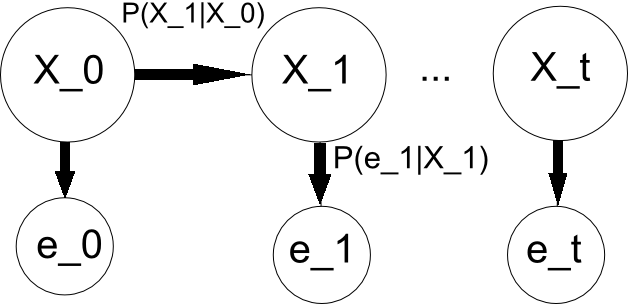
\includegraphics[width=1.2\textwidth]{HMM.png}
\caption{\label{fig:2x2 maze}Hidden Markov Model}
\end{figure}

\subsection{Maze Representation}

The maze is represented as a 2d character array wrapped in a maze class. Maze.java from the mazeworld assignment was modified to serve this purpose.Mazes are written as .maz files. Walls are represented with Xs and the colors red, green, blue, yellow are represented respectively as r,g,b,y.

\lstset{
numbers=none
}
\begin{lstlisting}
the following is a 4x4 maze with 3 walls:

rXbg
bXrX
ybrg
ybrg
\end{lstlisting}

\subsection{Transition Model}

The transition model is represented as a SxS Matrix where S is the number of state variables such that 
\begin{equation}
T_{ij} = P(X_t = j | X_{t-1} = i).
\end{equation}
By representing only the legal locations, time and memory is saved when calculating probability distributions. I used the la4j library to implement the Matrix. $T$ is generated automatically from a provided maze by the following method.

\lstset{
numbers=left
}
\begin{lstlisting}
//create the transition model from an ascii representation of the maze
//Each entry is: T_(ij) = P(X_(t) = j | X_(t-1) = i)
//
//SxS where S is the number of variables
//   X1        X2        X3
//X1[P(x1|x1)][P(x1|x2)][P(x1|x2)]...
//
//
//X2[P(x2|x1)][P(x2|x2)][P(x1|x2)]...
//
//
//X3[P(x3|x1)][P(x3|x2)][P(x1|x2)]...
//
//
//X4[P(x4|x1)][P(x4|x2)][P(x1|x2)]...
//...
private Matrix transitionModel(){
	
	//Key = set of locations Value = set of neighbors
	Hashtable<Integer, HashSet<Integer>> topography= getTopography();

	//size is number_of_variables x number_of_variables
	//i = Xt-1, j = Xt
	double[][] transition_probabilities = new double[variables.length][];

	//get P(X_t|X_t-1) for every variable pair
	int i=0;
	for (int variable: variables){
		transition_probabilities[i] = new double[variables.length];
		
		int j=0;
		for (int pastVariable: variables){
			
			//get P(X_t|X_t-1)
			//put it in the matrix
			transition_probabilities[i][j] = getTransitionProbability(pastVariable, variable, topography);
			j++;
		}
		i++;
	}
	return new Basic2DMatrix(transition_probabilities);
}
\end{lstlisting}

\subsection{Observation Model}

The observation model is represented as an array of SxS diagonal Matrices where S is the number of state variables such that
\begin{equation}
O_{i} = P(e_{t}|X_t = i)
\end{equation}. Each matrix corresponds to an emission variable and the contents of each matrix correspond to the probability of emission by the state variable.  I used the la4j library to implement the Matrices. 

$O$ is generated automatically from a provided maze by the following method.

\begin{lstlisting}
//build the observation model
//a list of matrices
//each matrix contains the probabilities that a state would emit the given observation variable
//the matrices are diagonal so that we can do matrix multiplication with the transition model
//SxS where S is the number of variables
//   X1  X2  X3  X4
// X1[p1][0 ][0 ][0 ]
// X2[0 ][p2][0 ][0 ]
// X3[0 ][0 ][p3][0 ]
// X4[0 ][0 ][0 ][p4]
private Matrix[] observationModel(){
	Matrix[] obs_mod = new Matrix[COLORS.length];
	
	
	int index=0;
	for (char color : COLORS){
		double[][] obs_matrix = new double[variables.length][];
		int i=0;
		for (int variable:variables){
			
			obs_matrix[i] = new double[variables.length]; //create an array full of 0s
			
			//if its a true reading
			if (maze.getChar(variable) == color){
				obs_matrix[i][i] = 1 - error_rate;
			}
			
			//if its an error
			else{
				obs_matrix[i][i] = error_rate/(COLORS.length-1);
			}
			i++;
			
		}
		obs_mod[index] = new Basic2DMatrix(obs_matrix);
		index++;
	}
	return obs_mod;
}
\end{lstlisting}

\subsection{Sensor Robot Representation}

SensorRobot.java extends the abstract class ProbabilisticReasoningAgent.java. The state is represented within ProbabilisticReasoningAgent.java as an ArrayList of Vectors of length S, where each index is the beliefstate at time t, S is the number of state variables and each entry is the probability of being at a particular location.

ProbabilistingReasoningAgent.java:
\begin{lstlisting}
//transition and observation models are represented as a lists of matrices, which are instantiated in concrete classes
	
	private Matrix transition_model; //#variables x #variables
	private Matrix[] observation_model; //list of diagonal matrices each matrix corresponds to an observation model for a particular observation value #vars x #vars

	public ArrayList<Vector> state; //probability distribution of state variables over time
\end{lstlisting}

SensorRobot contains representations of other useful bits of information in addition to beliefstate. It stores a char array of possible observation values. Since, ProbablisticReasoningAgent represents variables as ints, we pass the value of the color's index to it. And it stores the error rate of the sensors.

In addition to the above mentioned transition and observation model builders, SensorRobot contains generateRandomMoves(int num) and generateObservations(int[][] path, boolean toErrr). generateObservations returns a sequence of observations which may or may not contain errors proportional to the error rate depending on whether boolean toErrr is triggered.

SensorRobot.java
\begin{lstlisting}
//the set of robot moves
private static int[][] MOVES = {{1,0},{0,1},{-1,0},{0,-1}};

//the set of possible colors
private final char[] COLORS = {'r', 'g', 'b', 'y'};

//the max numbers of neighbors per location
private final double NUM_NEIGHBORS = 4;

//the sensor error rate
private double error_rate;

private Maze maze; //the robot knows the layout of the maze

public int[] variables; //the list of variables and their locations in the maze

//construct the HMM based off the maze
public SensorRobot(Maze m){
	
	maze = m;
	
	error_rate = .12;
	
	//Construct the models from the maze
	setVariables();
	setT(transitionModel());
	setO(observationModel());
	setState(variables.length);
}

//Generate a random set of moves -- a list of coordinates
public int[][] generateRandomMoves(int num){
	Random random = new Random();

	int[][] path = new int[num][];
	
	int var = variables[random.nextInt(variables.length)];
	path[0] = new int[]{var%maze.width, var/maze.width};

	for (int i=1; i< num; i++){
		int[] move = MOVES[random.nextInt(MOVES.length)];
		int newx = path[i-1][0] + move[0];
		int newy = path[i-1][1] + move[1];
		if(maze.isLegal(newx, newy)){
			path[i] = new int[]{newx, newy};
		}
		else{
			path[i] = path[i-1];
		}
	}
	return path;
}

//from a robot path, generate a list of observations
//parameters: boolean errr. if true the sensor will err
public int[] generateObservations(int[][] path, boolean toErrr){
	int[] observations = new int[path.length];
	
	if (!toErrr){
		int i=0;
		for (int[] location:path){
			char c = maze.getChar(location[0], location[1]);
						
			observations[i] = getCharInt(c);
			i++;
		}
		return observations;
	}

	Random random = new Random();
	
	int i=0;
	for (int[] location:path){
		char c = maze.getChar(location[0], location[1]);
		
		double error = random.nextDouble();
		System.out.println(error + " " + error_rate);
		//get the correct observation
		int charval = getCharInt(c);
	
		//Generate a random error
		if (error < error_rate){
			int errorchar = charval;
			while (errorchar == charval){
				errorchar = random.nextInt(COLORS.length-1);
			}
			observations[i] = errorchar;
		}
		else{
			observations[i] = charval;
		}
	
	
		i++;
	}
	return observations;
}
\end{lstlisting}

\section{Filtering}

Filtering is the process of computing the belief state at the current time t, given previous observations -- that is computing expression (7). However, it is best to look at filtering as a process of updating the belief state. This way, the filtering algorithm needs not compute the belief state from 0:t every time the agent wants to compute its current belief state, but rather build off previous calculations. Thus we rewite expression (7) as a function of an updating filtering algorithm:

\begin{equation}
P(X_{t+1}|e{1:t+1}) = f(e_{1:t+1},P(X_t|e_{1:t}))
\end{equation}

\subsection{Forward Algorithm}

The Forward algorithm can be seen as a recursive algorithm which teases the $P(X_{t+1}|e{1:t+1})$ into something calculatable, by eumerating it into a set of expressions defined by the models $T$ and $O$.
\begin{equation}
\begin{array}{l@{}l}
P(X_{t+1}|e_{1:t+1})  
&{}= P(X_{t+1}|e_{1:t}, e_{t+1}) (splitting the term)\\
&{}= \alpha P(e_{t+1}|X{t+1}, e_{1:t})P(X_{t+1}|e{t+1})  (Bayes)\\
&{}= \alpha P(e_{t+1}|X{t+1})P(X_{t+1}|e{1:t})   (Markov Assum.)\\
&{}= \alpha P(e_{t+1}|X{t+1}) \sum_{\substack{x_t}} P(X_{t+1}|x_t,e{1:t})P(x_t|e_{1:t})(Joint Probability)\\
&{}= \alpha P(e_{t+1}|X{t+1}) \sum_{\substack{x_t}} P(X_{t+1}|x_t)P(x_t|e_{1:t})(Markov Assum.)\\
...
\end{array}
\end{equation}
The filtering expression has been enumerated from $P(X_{t+1}|e_{1:t+1})$ to several terms held in the model  ($P(e_{t+1}|X{t+1}) = O_i$ and $P(X_{t+1}|x_t) = T_{ij}$) and $\alpha$, a normalizing constant. As for $P(x_t|e_{1:t})$, which is not in the model, it is the belief state at the previous time slice! If it is defined as $forward_{1:t}$, the value returned from a previous iteration, then filtering can be defined as a recursive algorithm which computes the distribution over state variables from time 1 to t. This is the Forward algorithm:

\begin{equation}
\begin{array}{l@{}l}
forward_{1:t+1}
&{}= \alpha P(e_{t+1}|X{t+1}) \sum_{\substack{x_t}} P(X_{t+1}|x_t)P(x_t|e_{1:t})\\
&{}= \alpha O_{t+1} T^T forward_{1:t}(matrix multiplication)\\
&{}= \alpha FORWARD_{1:t+1}(forward_{1:t}, e_{t+1})(substitution)\\
\end{array}
\end{equation}

The Forward algorithm's time complexity grows linearly with time. Since, it only needs to keep track of the previous step it only requires constant space.//

In my implementation of the forward algorithm, I used matrices to represent $T$ and $O$. 

\begin{lstlisting}

//Compute the Belief State at time t: P(State_0:t|sequenceOfObservations_1:t)
//
//returns a sequence of belief states at each step of the observation
//parameters: int[] obs is the sequence of observations
public ArrayList<Vector> filter(int[] obs){
	ArrayList<Vector> forward_vector = new ArrayList<Vector>();
	forward_vector.add(state.get(0));
	return forward(forward_vector.get(0), obs, forward_vector, 0, false);
}

private ArrayList<Vector> forward(Vector prev_forward, int[] obs,  ArrayList<Vector> state_to_t, int t, boolean isFB){
	//Base Case
	if (t >= obs.length){
		return state_to_t;
	}

	//Recursive Case		
	Vector current = null;
	//not used for forward backward, normalize
	if (isFB == false){
		//new matrix = a*O*Transpose(T)*(prev_forward)
		current = normalize(getO(obs[t]).multiply(getT()).multiply(prev_forward));
	}
	else{
		//new matrix = a*O*Transpose(T)*(prev_forward)
		current = getO(obs[t]).multiply(getT()).multiply(prev_forward);
	}
	
	state_to_t.add(current);
	
	//recursiveCall
	return forward(current, obs, state_to_t, t+1, isFB);
}
\end{lstlisting}

\subsection{Filtering Results}

The following is a table of the probability distribution over locations. Each cell in the table represents a location at a specified time. At time t=0, the distribution is uniform, representing that the robot has no idea where it is. At time t=1 the robot senses the presence of red and updates the belief state and so on.

\lstset{
numbers=none
}
\begin{lstlisting}
Maze:
rg
by

\end{lstlisting}

\begin{figure}[H]
\centering
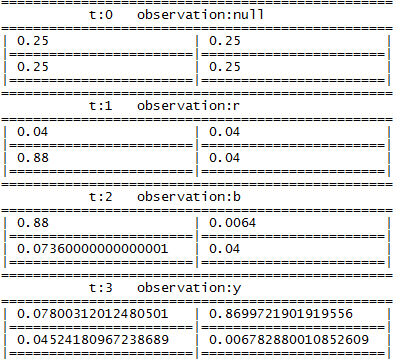
\includegraphics[width=1\textwidth]{2x2Filtertext.png}
\caption{\label{fig:2x2 maze}Table of probability distribution over locations}
\end{figure}


The following is a graphical presentation of the same results as Figure 1. Balkcom's head represents the true location of the robot at time t. The black bars represent the probability distribution at each location. The hight of the bar represents the probability value. 1 = a bar that spans the entire hight of a tile. .5 = a bar that spans half the hight of a tile and so on.

\begin{figure}[H]
\centering
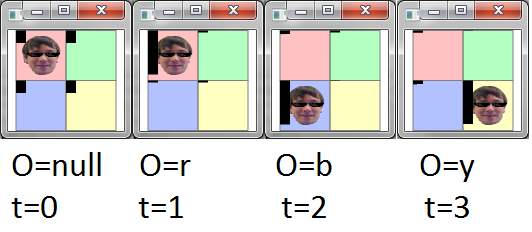
\includegraphics[width=1\textwidth]{2x2Filter.png}
\caption{\label{fig:2x2 maze}2x2 Maze Filtering $X_{0:t}$}
\end{figure}

However, Filtering is not always accurate. Sometimes the most probable location given a sequence of observations is not the actual location! At times t=8 and t=9 the most probable location is different than the actual location. At t=8, this is because the red tile between the walls has a higher probability (.5)of transitioning into itself than to the red tile adjacent it (.25). Thus, the calculation at t=8 carries over to t=9.
\begin{figure}[H]
\centering
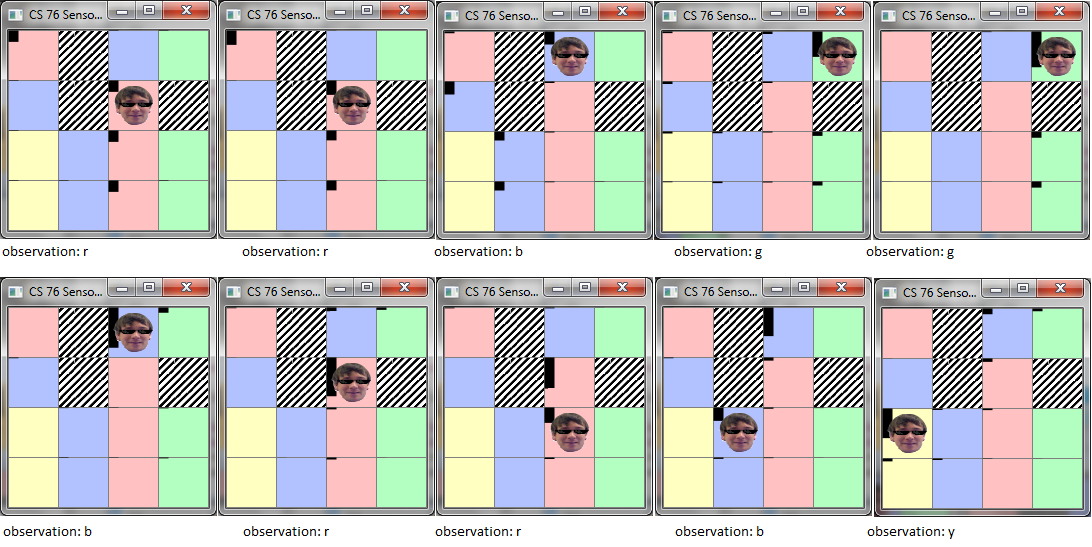
\includegraphics[width=1\textwidth]{4x4WallMazeFilter.png}
\caption{\label{fig:4x4 maze}4x4 Maze Filtering $X_{1:t}$}
\end{figure}


\section{Smoothing}

Smoothing is the process of computing the belief state at a past time k, given every observation up to the current time t where $0<k<t$:
\begin{equation}
P(X_{k}|e_{1:t})
\end{equation}

\subsection{Forward-Backward Algorithm}


Expresssion 13 can be split into two expressions, one which is the Forward algorithm the other is the Backward algorithm:

\begin{equation}
\begin{array}{l@{}l}

P(X_{k}|e_{1:t}) 
&{}= \alpha P(X_{k}|e_{1:k})P(e_{k+1:t}|X_k, e_1:k)(Bayes)\\
&{}= \alpha P(X_{k}|e_{1:k})P(e_{k+1:t}|X_k)(condit. Indepenance see fig.1)\\
&{}= \alpha forward_{1:k} (x) backward_{k+1:t}

\end{array}
\end{equation}

Whereas the forward algorithm computes the probability distribution over state variables given a sequence of observations, the backwards algorithm computes the probability of a sequence of observations given probability distributions over state variables. 

\begin{equation}
\begin{array}{l@{}l}

P(e_{k+1:t}|X_k) 
&{}= \sum_{\substack{x_{k+1}}} P(e_{k+1:t}|X_k, x_{k+1})P(x_{k+1}|X_k)(Joint Probability)\\
&{}= \sum_{\substack{x_{k+1}}} P(e_{k+1:t}|x_{k+1})P(x_{k+1}|X_k)(condit. Independance see fig.1)\\
&{}= \sum_{\substack{x_{k+1}}} P(e_{k+1},e_{k+2:t}|x_{k+1})P(x_{k+1}|X_k)(seperating observations)\\
&{}= \sum_{\substack{x_{k+1}}} P(e_{k+1}|x_{k+1})P(e_{k+2:t}|x_{k+1})P(x_{k+1}|X_k)\\&{}(condit. Indp Of e_{k+1} And e{k+2} Given x_{k+1})\\
...

\end{array}
\end{equation}

Like in the forward algorithm, the expression has been enumerated from $P(e_{k+1:t}|X_k)$ to several termsin the transition and observation models ($P(e_{k+1}|x_{k+1}) = O_i$ and $P(x_{k+1}|X_k) = T_{ij}$). As for $P(e_{k+2:t}|x_{k+1})$, which is not known in the models, it is expression at the next time step! Thus, the backward algorithm can be defined as a recursive algorithm that probagates its message, $backward_{k+1:t}$, backwards from t to k:

\begin{equation}
\begin{array}{l@{}l}
backward_{k+1:t}
&{}= \sum_{\substack{x_{k+1}}} P(e_{k+1}|x_{k+1})P(e_{k+2:t}|x_{k+1})P(x_{k+1}|X_k)\\
&{}= TO_{k+1} backward_{k+2:t}(matrix multiplication)\\
&{}= BACKWARD_{k+1:t}(backward_{k+2:t}, e_{k+1})(substitution)\\
\end{array}
\end{equation}

The forwardbackward algorithm is much more accurate than just the forward algorithm. However, the forwardbackward algorithm is not as memory efficient. Its space complexity is $O(ft)$ where $f$ is the size of the forward message and $t$ is the number of time steps.


In my implementation of the forwardbackward algorithm, I used matrices


\lstset{
numbers=left
}
\begin{lstlisting}

//Compute the Belief State at time k: P(State_0:k|sequenceOfObservations_1:k)*PsequenceOfObservations_k+1:t|State_k+1:t)
//
//returns a sequence of belief states at each step of the observation
//parameters: int[] obs is the sequence of observations
public ArrayList<Vector> smoothing(int[] obs){
	return forwardBackward(obs);
}

//Compute the Belief State at time k: P(State_0:k|sequenceOfObservations_1:k)*PsequenceOfObservations_k+1:t|State_k+1:t)
//
//returns a sequence of belief states at each step of the observation
//parameters: int[] obs is the sequence of observations
private ArrayList<Vector> forwardBackward(int[] obs){
	
	ArrayList<Vector> forward_vectors = new ArrayList<Vector>();
	forward(state.get(0), obs, forward_vectors, 0, true);
	
	ArrayList<Vector> backward_vectors = new ArrayList<Vector>();
	
	//backwards algorithm starts with a vector filled with ones
	double[] firstBack = new double[state.get(0).length()];
	Arrays.fill(firstBack, 1.0);
	backward_vectors.add(0,new BasicVector(firstBack));
	
	backward(backward_vectors.get(0), obs, obs.length-1, backward_vectors, true);
	
	for (int i=0; i<obs.length; i++){
		state.add(normalize(forward_vectors.get(i).hadamardProduct(backward_vectors.get(i))));
	}
	return state;
}

private ArrayList<Vector> backward(Vector prev_backward, int[] obs, int t, ArrayList<Vector> state_to_1, boolean isFB){
	//Base Case
	if (t < 1){
		return state_to_1;
	}

	//Recursive Case
	
	Vector current = null;
	if (isFB != true){
		//new matrix = a*T*O*(prev_backward)
		current = normalize(getT().multiply(getO(obs[t])).multiply(prev_backward));
	}
	else{
		//new matrix = T*O*(prev_backward)
		current = getT().multiply(getO(obs[t])).multiply(prev_backward);
	}
	
	state_to_1.add(0, current);
	
	//recursiveCall
	return backward(current, obs, t-1, state_to_1, isFB);
}
\end{lstlisting}

\subsection{Smoothing Results}


The following is a table of the probability distribution over locations. Each cell in the table represents a location at a specified time. At time t=0, the distribution is uniform, representing that the robot has no idea where it is. At time t=1 the robot senses the presence of red and updates the belief state and so on.

Excluding the belief states at time = 0 and time = t, the forward backward algorithm is much more accurate than the forward algorithm. At time = 0 and time = t, the distributions returned from forward-backward and forward are exactly the same. Looking at Figures 1. and 5. shows this is true.
\begin{figure}[H]
\centering
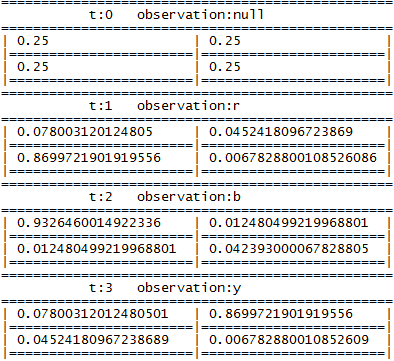
\includegraphics[width=1\textwidth]{2x2Smoothingtext.png}
\caption{\label{fig:2x2 maze}2x2 ForwardBackward}
\end{figure}

The following is a graphical presentation of the same results as Figure 5.

\begin{figure}[H]
\centering
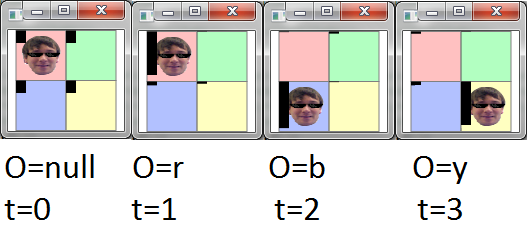
\includegraphics[width=1\textwidth]{2x2Smoothing.png}
\caption{\label{fig:2x2 maze}2x2 ForwardBackward}
\end{figure}

\section{Forward vs. ForwardBackward}

\subsection{Accuracy}

In many cases, filtering makes mistakes. At time k, it makes many more mistakes than smoothing. For example, at time = 8 the robot believes it is on the red tile between the walls. This is because the filtering gets no information from observations made after k.

\begin{figure}[H]
\centering
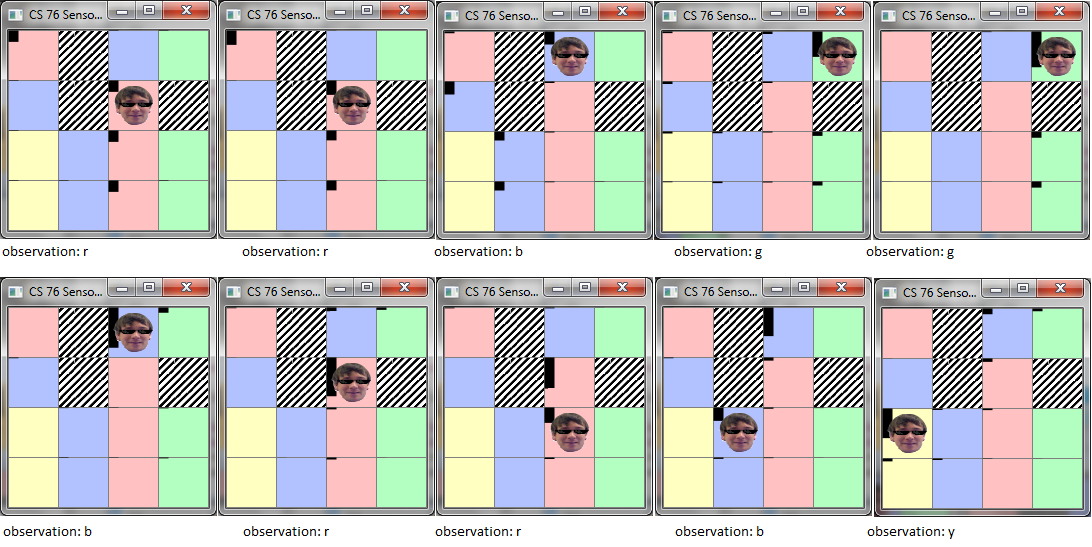
\includegraphics[width=1\textwidth]{4x4WallMazeFilter.png}
\caption{\label{fig:2x2 maze}4x4maze filtering: pobability distribution of locations}
\end{figure}

\begin{figure}[H]
\centering
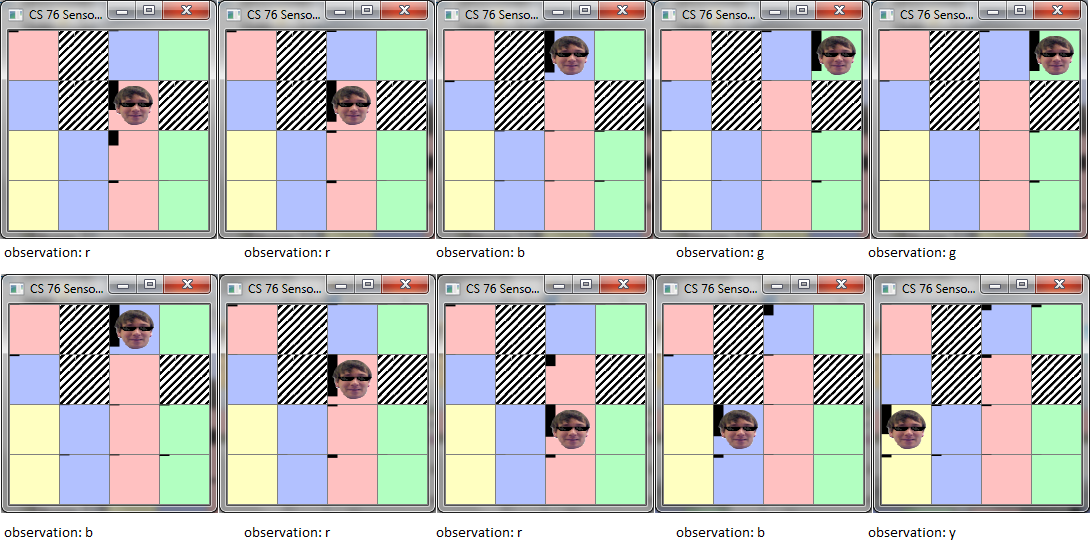
\includegraphics[width=1\textwidth]{4x4WallMazeSmoothing.png}
\caption{\label{fig:2x2 maze}4x4maze smoothing: pobability distribution of locations}
\end{figure}

\subsection{Dealing with a Noisy Channel}

Since the sensors of the robot are prone to error, it is important to have algorithms which can deal with error. This error is treated as a noisy channel, and the error rate is accounted for in the observation model. First, in figures 11 and 12, results from filtering and smoothing respectively of a sequence of observations with no error are shown.

\begin{figure}[H]
\centering
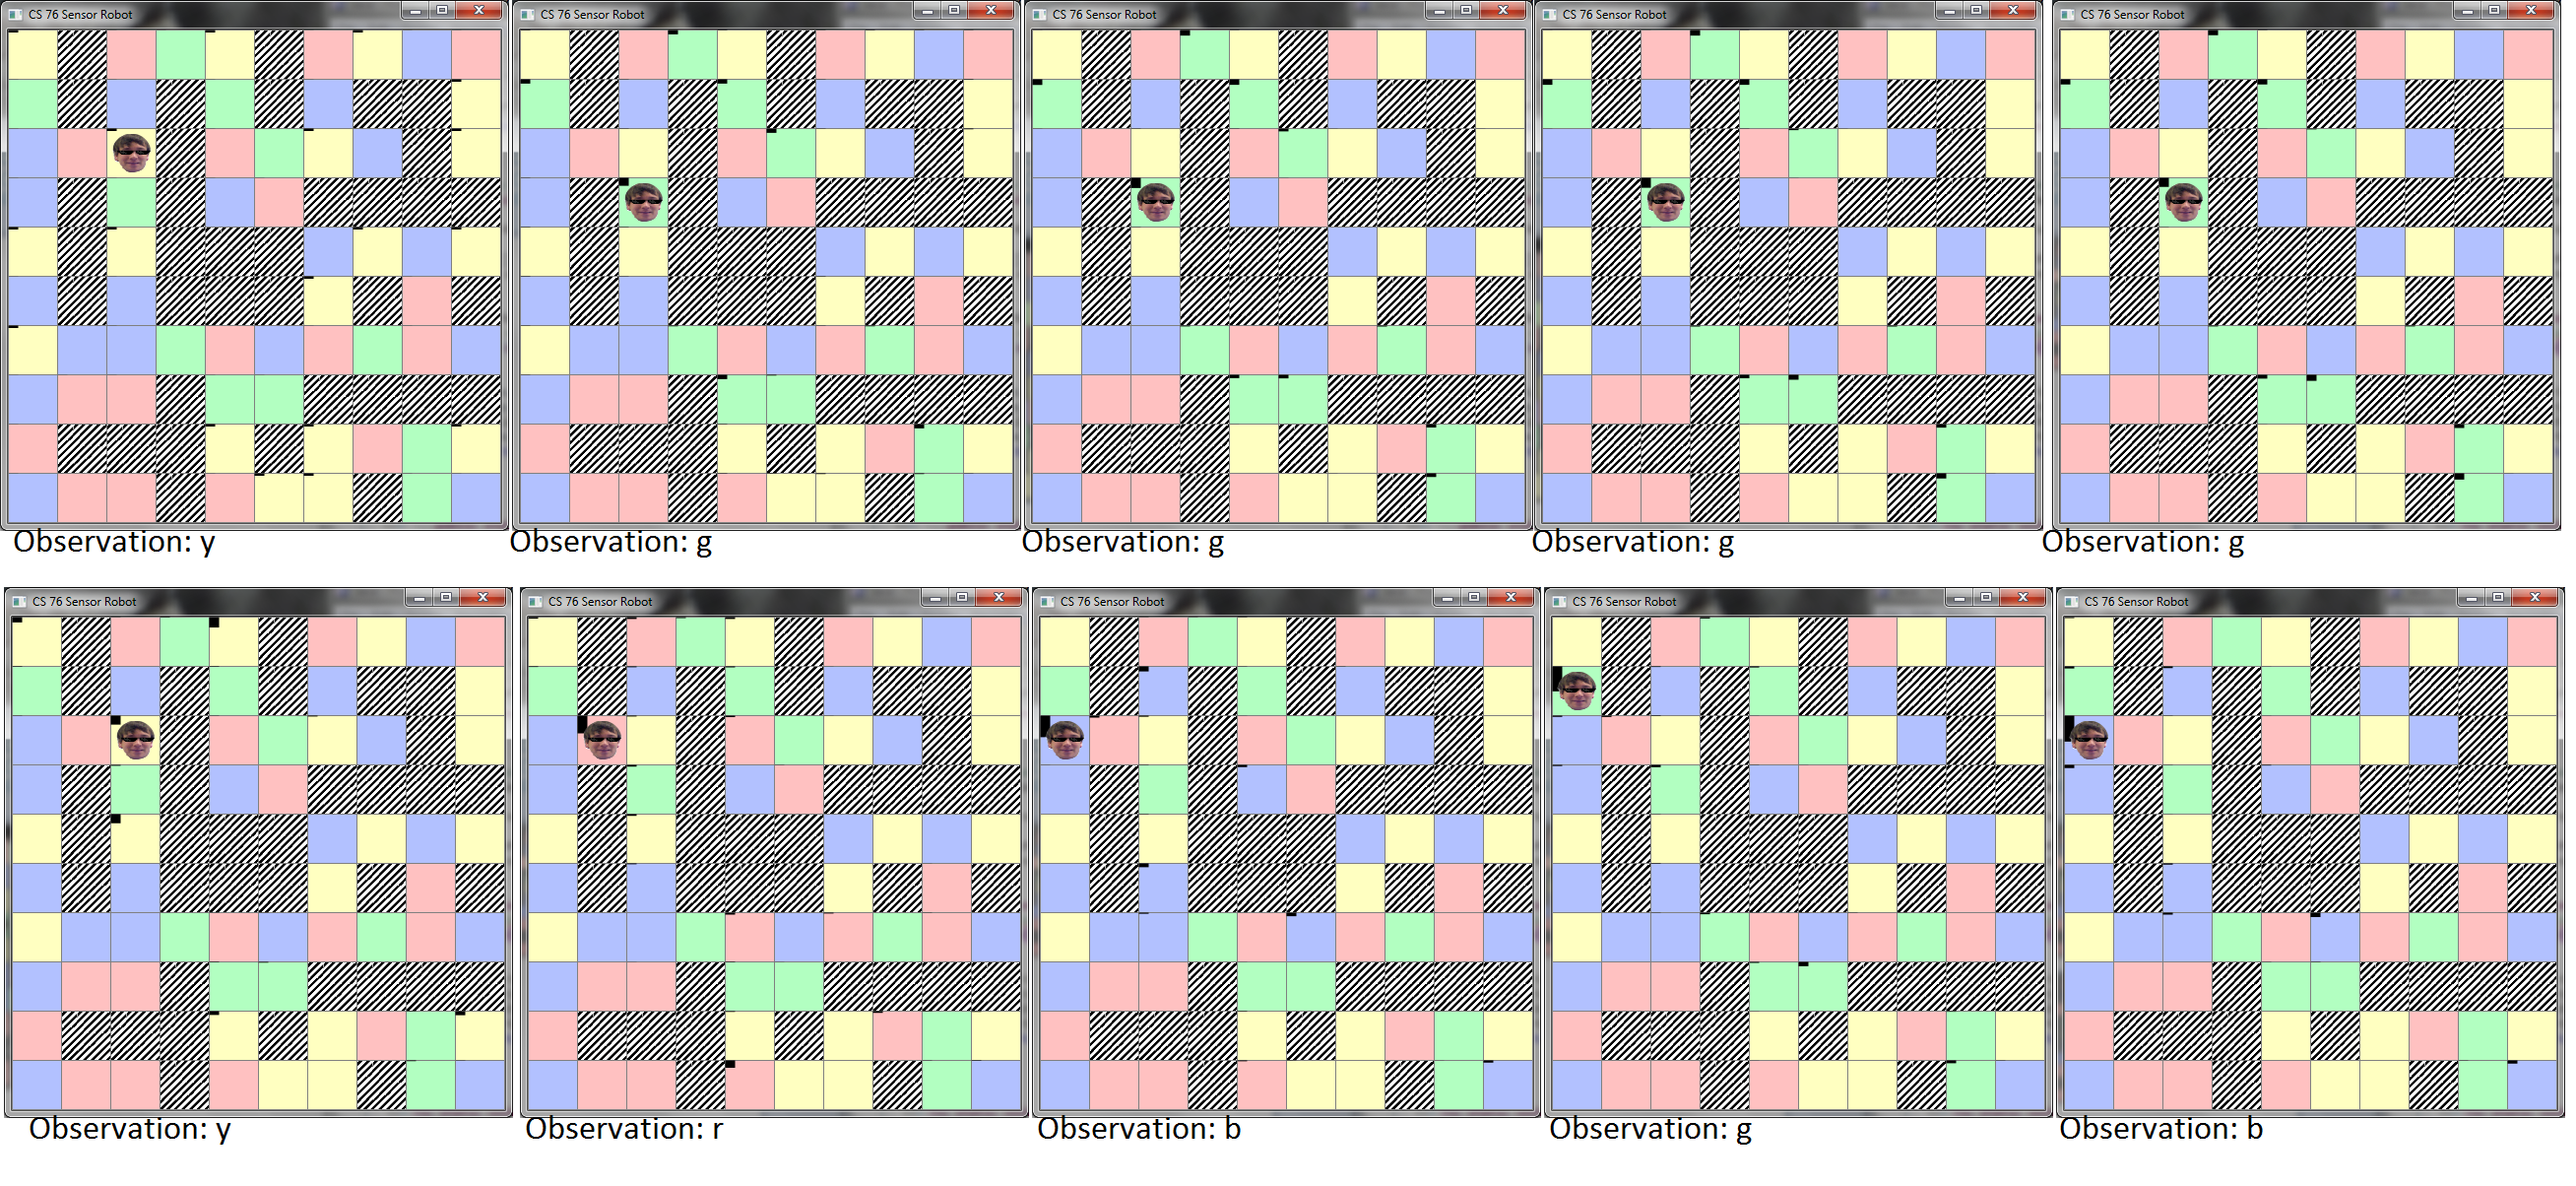
\includegraphics[width=1.2\textwidth]{4x4WallMazeFiltering_no_mistake.png}
\caption{\label{fig:2x2 maze}Filtering: no errors in observation sequence}
\end{figure}

\begin{figure}[H]
\centering
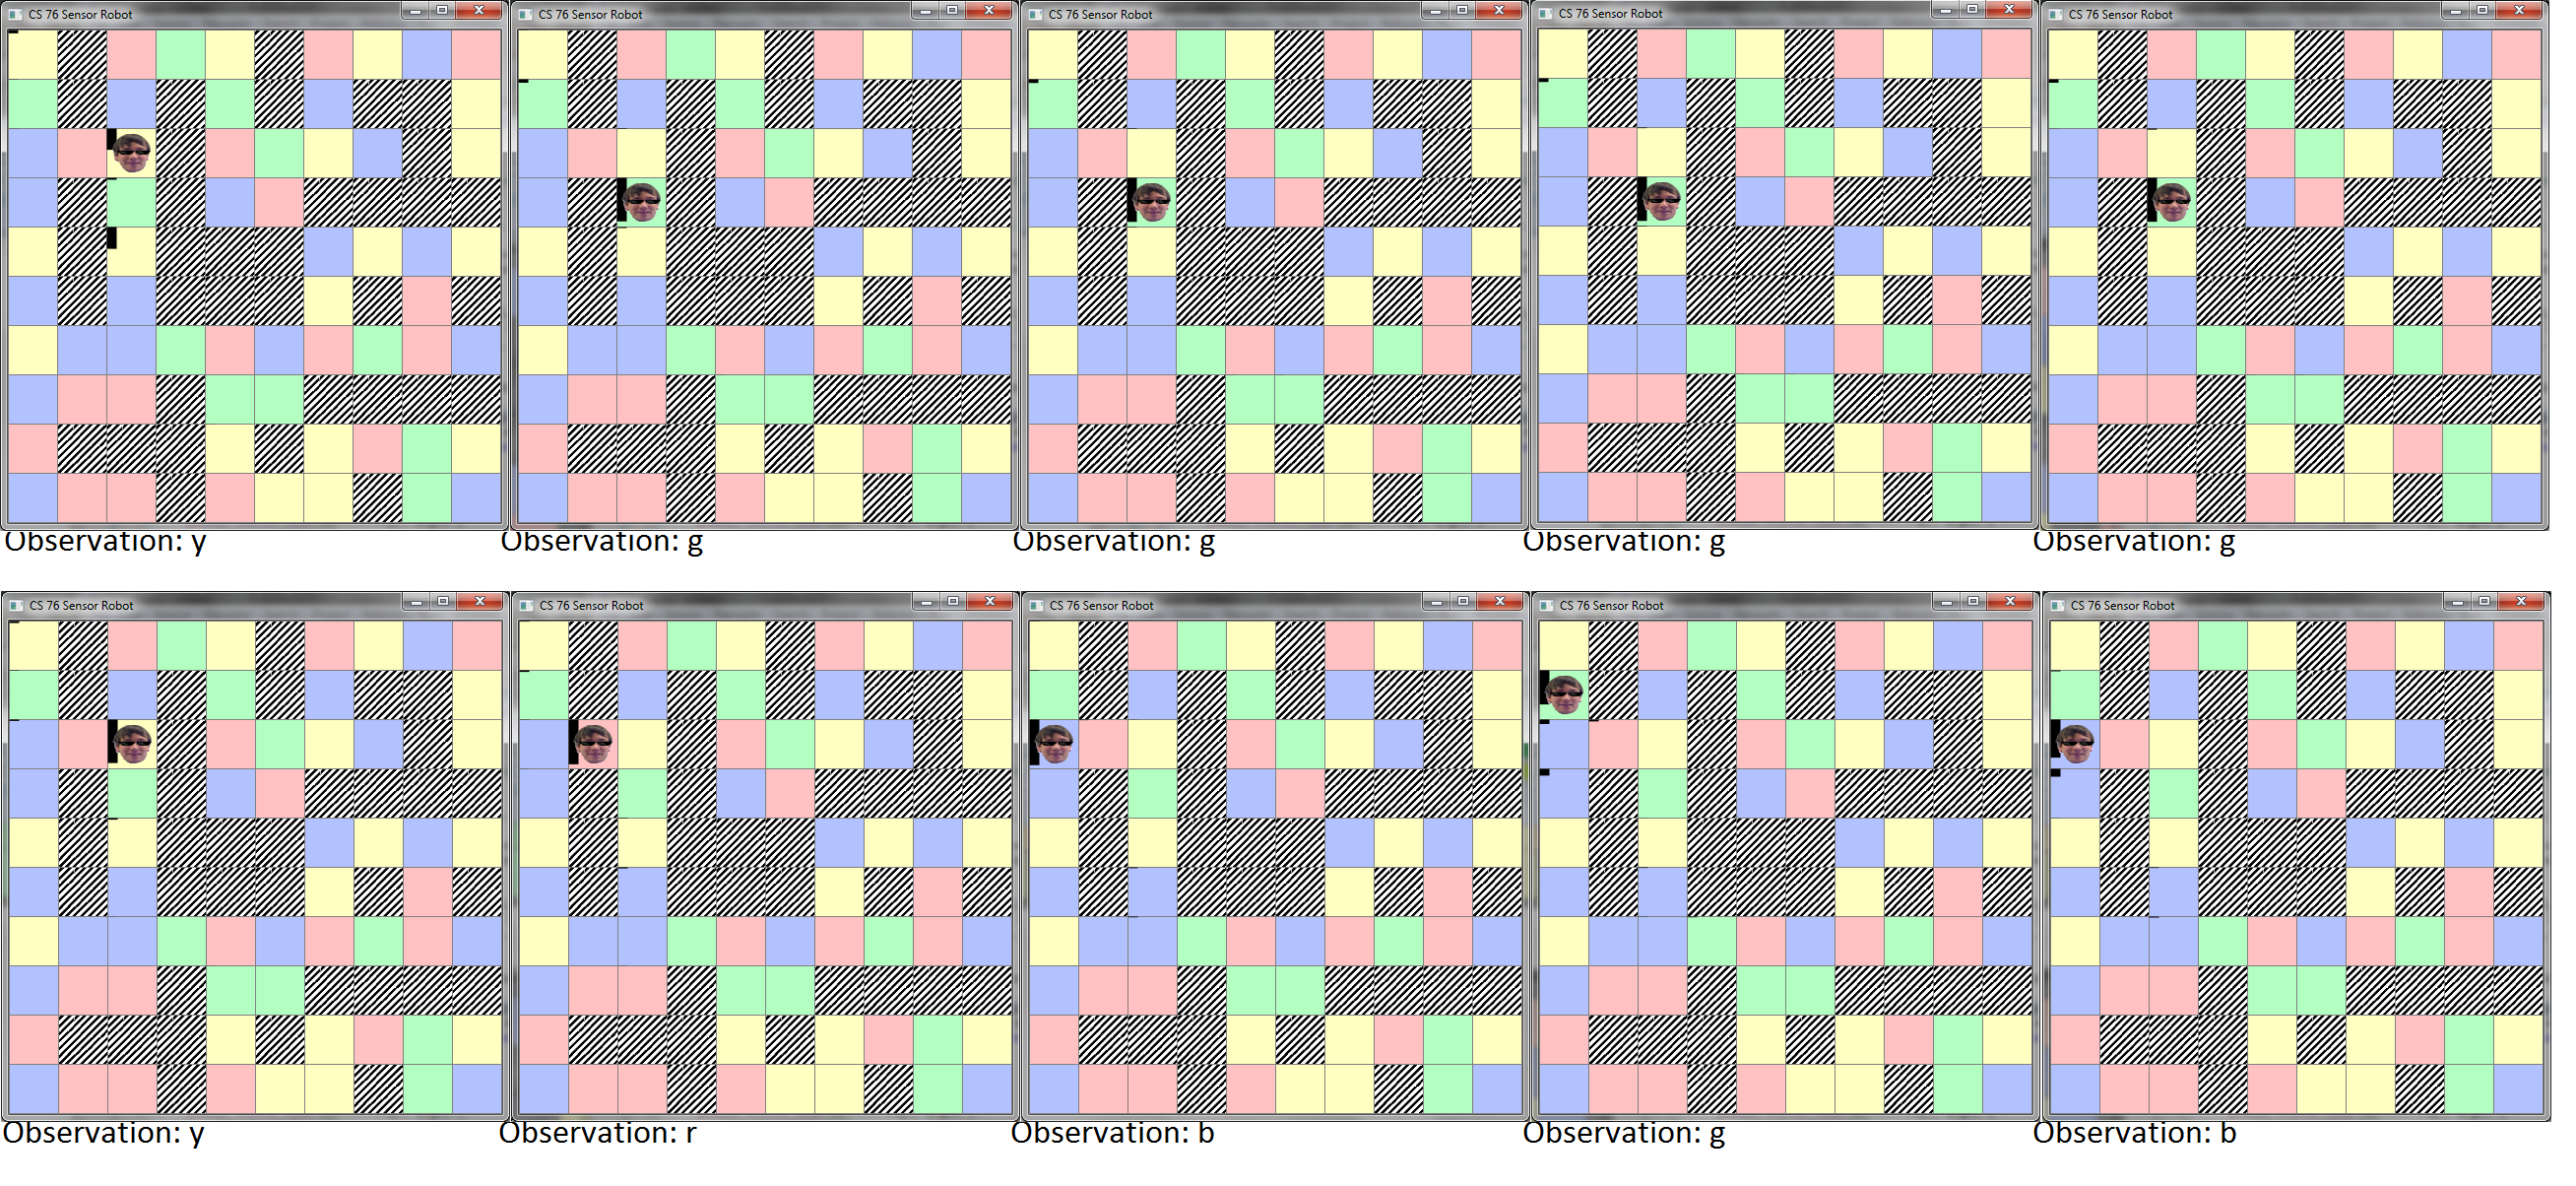
\includegraphics[width=1.2\textwidth]{4x4WallMazeSmoothing_no_mistake.png}
\caption{\label{fig:2x2 maze}Smoothing: no errors in observation sequence}
\end{figure}

However, in figures 13 and 14 there is an error at time = 1. Instead of reading yellow, the robot reads red. With filtering, not only, does the distribution not make an accurate inference afterword, but the distribution is not even clustered around the actual distribution. However, with smoothing, the distribution recovers after the erronious sensor reading. And, even at the erronious time step, the distribution is clustered around the actual location.

\begin{figure}[H]
\centering
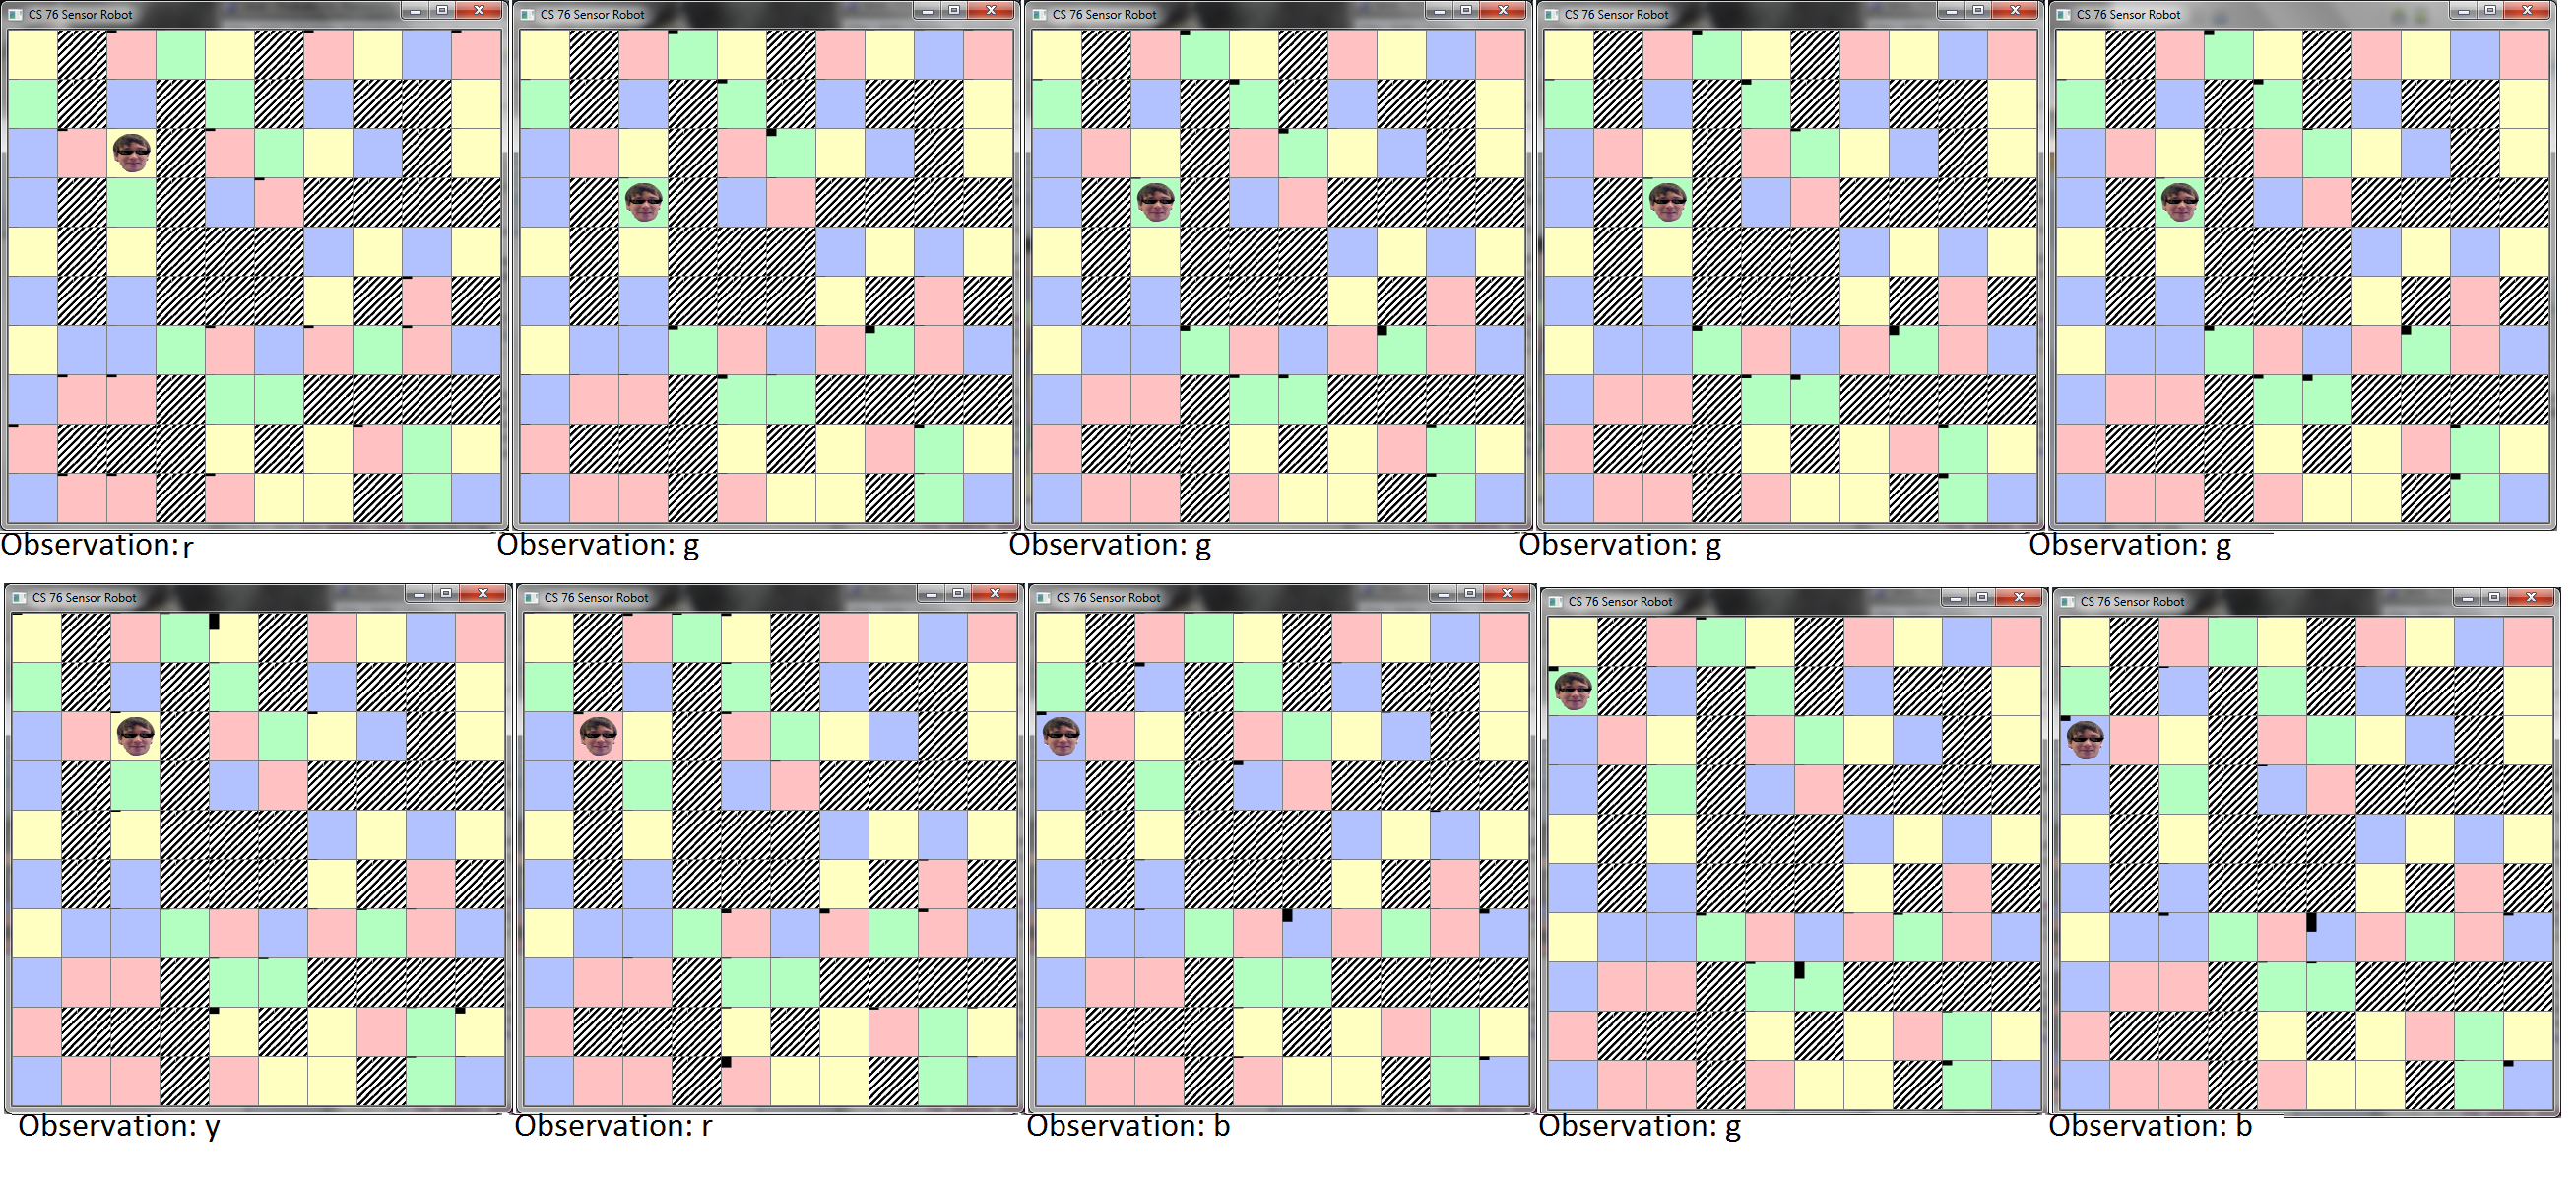
\includegraphics[width=1.2\textwidth]{4x4WallMazeFiltering_mistake_at1.png}
\caption{\label{fig:2x2 maze}Filtering: 1 Error at time t=1}
\end{figure}

\begin{figure}[H]
\centering
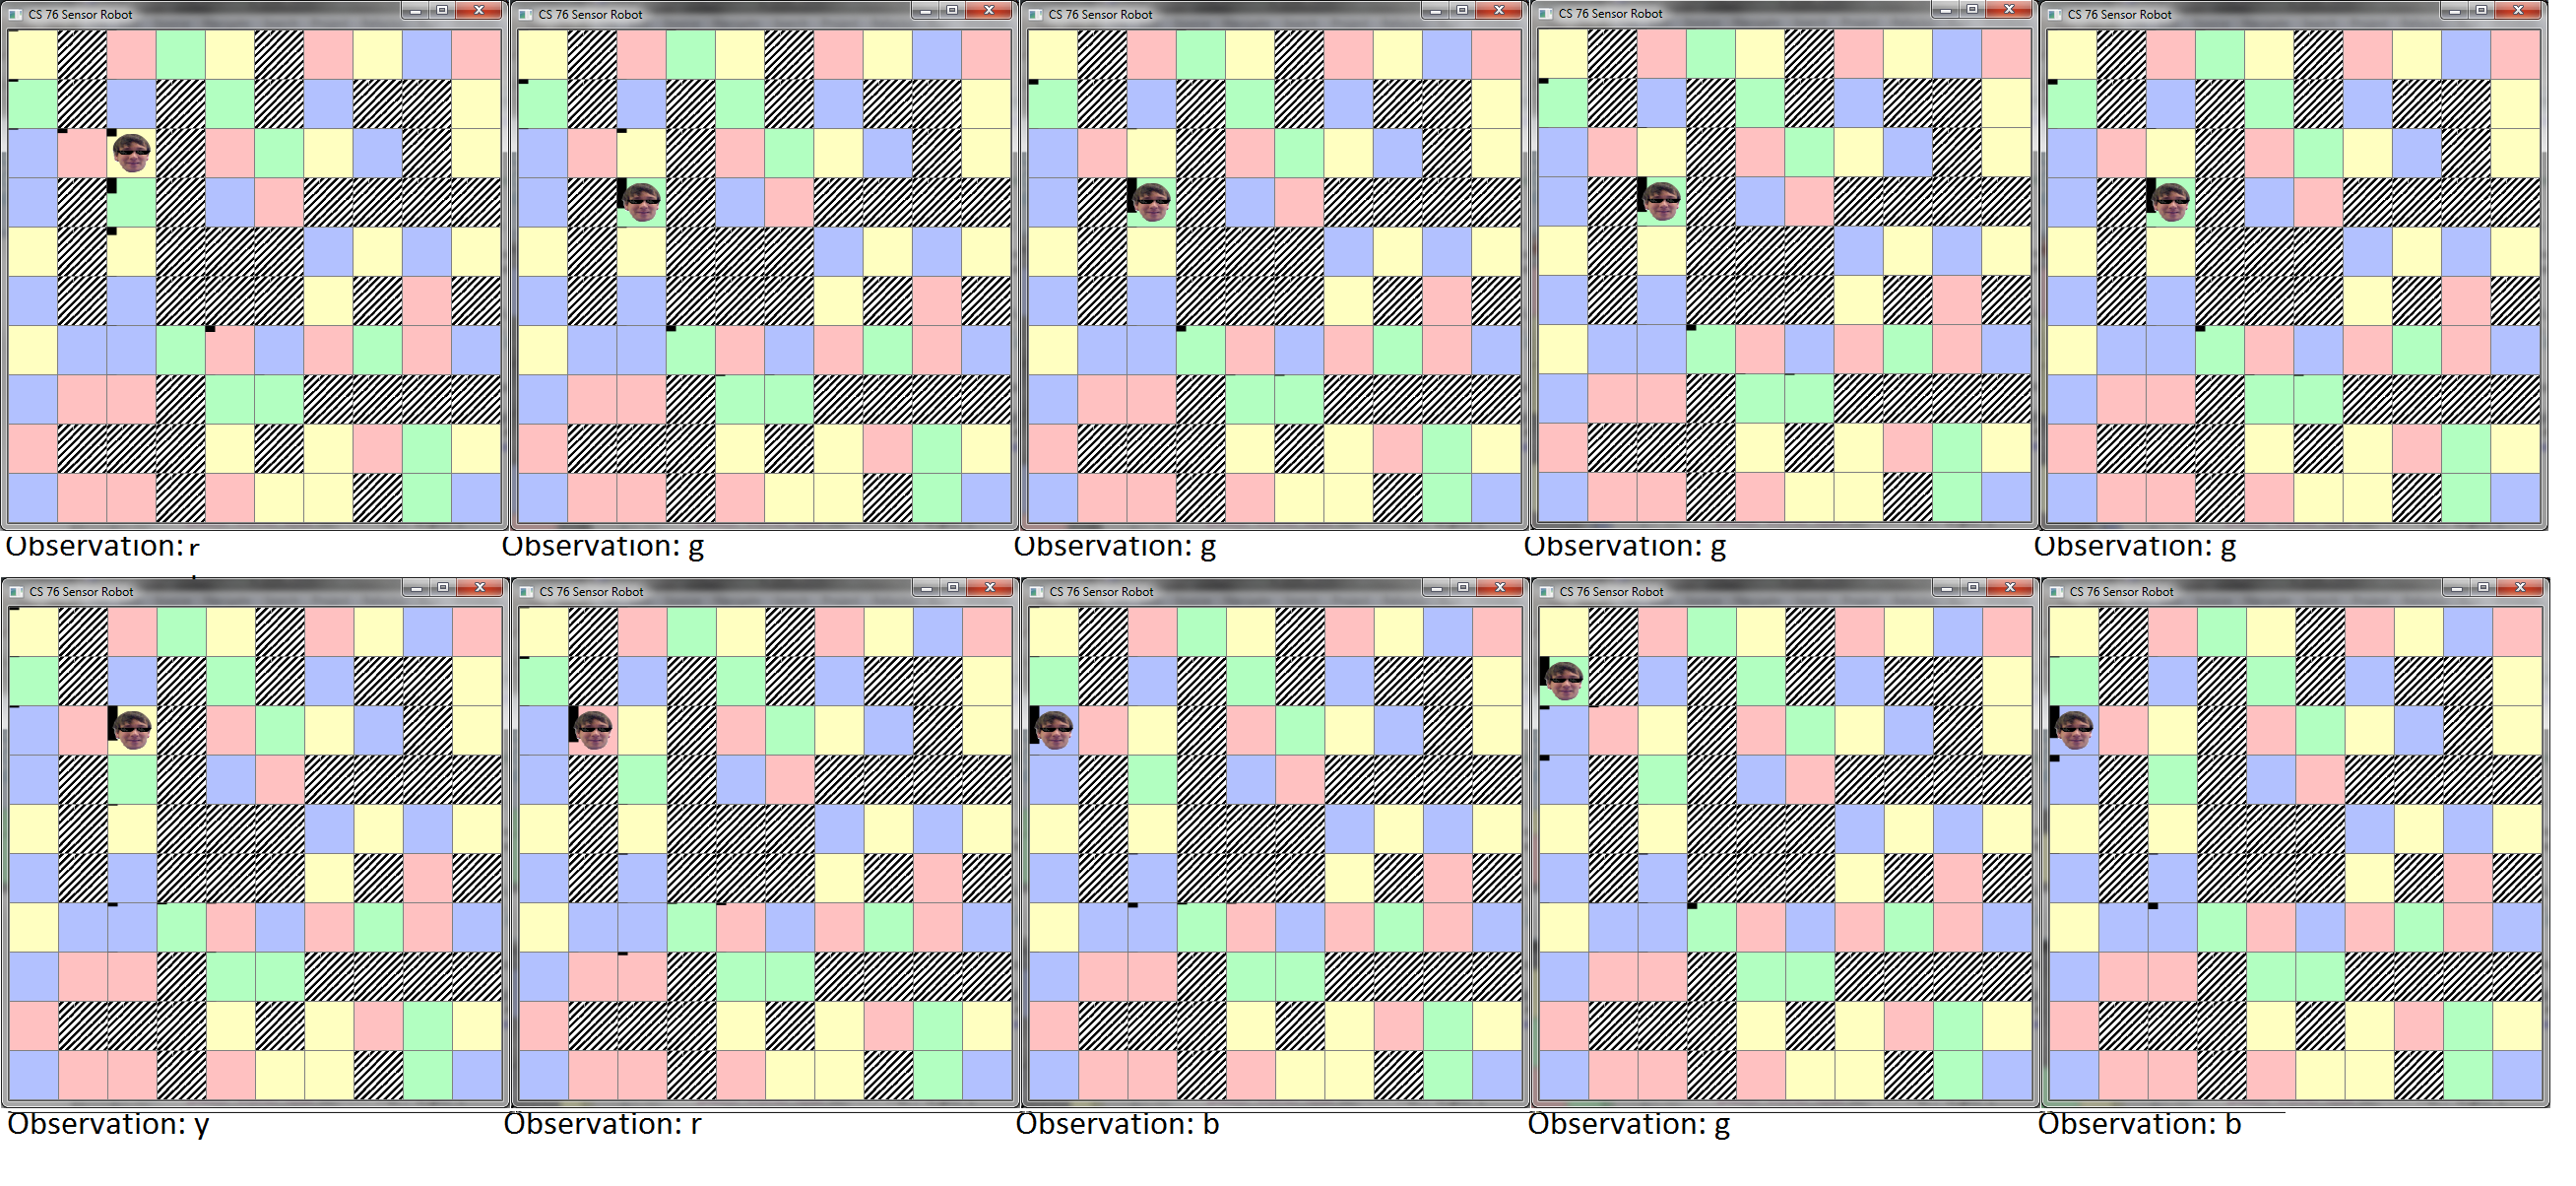
\includegraphics[width=1.2\textwidth]{4x4WallMazeSmoothing_mistake_at1.png}
\caption{\label{fig:2x2 maze}Smoothing: 1 Error at time t=1}
\end{figure}

My results suggest that filtering should be used only to update and predict states in the future. To infer the belief state at previously observed timeslices, Forward-Backward should be used.

\section{Most Likely Path}

To calculate the most likely path taken, the robot must find the most likely path to the most likely variable at time t+1.

\begin{equation}
\begin{array}{l@{}l}
max_{x_{1:t}} P(x_{1:t},X{t+1}|e_{1:t+1})
\end{array}
\end{equation}

\subsection{Virterbi Algorithm}

The Viterbi Algorithm computes expression 17. An interesting perspectve of the Viterbi Algorithm is to view it as modified breadth first search, where the depth is defined by time,  the goal is defined by $argmax_x P(X_{t+1}|e_{t+1})$, and the get neighbors function is a modified filtering update function.Thus:

\begin{equation}
\begin{array}{l@{}l}
max_{x_{1:t}} P(x_{1:t},X{t+1}|e_{1:t+1})\\
= \alpha P(e_{t+1}|X_{t+1})(P(X_{t+1}|x_t)max_{x1:t-1}P(x_{1:t-1}), x_t|e_{1:t}) 
\end{array}
\end{equation}

Viterbi, like filtering takes linear time. But unlike filtering, which only requires constant space, Viterbi's memory usage grows linearly with time, because it has to keep track of back pointers.

\lstset{
numbers=left
}
\begin{lstlisting}
//Compute the Most Likely Path through the state space given a sequence of observations
//
//I didn't use la4j in Viterbi
//
//returns an array of ints representing state variables
//parameters: int[] obs is the sequence of observations
public int[] mostLikelySequence(int[] obs){
	//initialize state at t0: 
	double[] start_probability = new double[transition_model.rows()];
	Arrays.fill(start_probability, 1);
	return viterbi(obs, 0, start_probability, new int[obs.length][]);
}

//Recursive Viterbi: At time t, find the most probable path for every state variable from t-1 to t
//
//returns the most likely path through the state space
//parameters: int[] obs the sequence of observations, int t the current time slice t,
//double[] past_probabilities the probability distribution of state variables at time t-1, int[][] viterbiPath set of backPointers for every t
private int[] viterbi(int[] obs, int t, double[] past_probabilities, int[][] viterbiPath){
	
	//Base Case
	
	//backtrack through the set of backpointers
	if (t >= obs.length){
		return backtracking(viterbiPath, past_probabilities);
	}
	
	//Recursive Case
	
	//get Ot
	Matrix obs_mod = observation_model[obs[t]];
	
	//new set of backpointers and set of probability distribution over state variables
	int[] subPath = new int[past_probabilities.length];
	double[] current_probabilities = new double[past_probabilities.length];
	
	//for every variable x_t, get the max P(x1_t|X_t-1)
	for (int state_variable_current=0; state_variable_current<transition_model.rows(); state_variable_current++){
		
		int max = 0; //the max variable
		double max_prob = 0; //the max probability
		double full_prob = 0;
		
		//for every variable x_t-1
		for (int state_variable_past=0; state_variable_past<transition_model.columns(); state_variable_past++){
			
			double probabilityOfstate_variable = transition_model.get(state_variable_current, state_variable_past)*obs_mod.get(state_variable_current, state_variable_current)*past_probabilities[state_variable_past];
							
			if (probabilityOfstate_variable > max_prob){
				max = state_variable_past;
				max_prob = probabilityOfstate_variable;
			}
			full_prob += probabilityOfstate_variable;

		}
		
		//add backpointer
		subPath[state_variable_current] = max;
		
        //The On the last iteration, get the combined probability of a state.
        //this way viterbi chooses the most likely path to the most likely state at t
		if (obs.length-1 == t){
			System.out.println(state_variable_current + " " + max_prob);
			//add max P(x_t|X_t-1)
			current_probabilities[state_variable_current] += full_prob;
		}
		else{
			current_probabilities[state_variable_current] = max_prob;
		}

	}
	viterbiPath[t] = subPath;
	
	//recurse
	return viterbi(obs, t+1, current_probabilities, viterbiPath);
}

//Backtrack through the most likely path
//at each time t, a variable points backward to which state most likely transitioned to it
//
//returns int[] path. an array of ints representing the most likely path through state space
//parameters: viterbiPath is the set of backpointers at every time t, double[] past_probabilities the distribution of state variables over time t
private int[] backtracking(int[][] viterbiPath, double[] past_probabilities){
	//System.out.println(past_probabilities[26] + " " + past_probabilities[7] + " " + past_probabilities[9]+ " " + past_probabilities[13]+ " " + past_probabilities[16]+ " " + past_probabilities[20] + " " + past_probabilities[35]);
	int[] path = new int[viterbiPath.length];
	
	//Find the most probable state at time t
	//we will backtrack through the path that let to this state
	int max = 0;
	double max_prob = 0;
	for (int j=0; j<past_probabilities.length; j++){
		if (max_prob<past_probabilities[j]){
			max = j;
			max_prob = past_probabilities[j];
		}
	}
	
	
	path[viterbiPath.length-1] = max;
	return backtracking(viterbiPath, viterbiPath.length-1, path);
}

//Backtrack through the most likely path
//at each time t, a variable points backward to which state most likely transitioned to it
//
//returns int[] path
//parameters: viterbiPath is the set of backpointers at every time t, 
private int[] backtracking(int[][] viterbiPath, int t, int[] path){
	
	//Base Case
	if (t == 0){
		return path;
	}
	
	//recursive case
	path[t-1] = viterbiPath[t][path[t]];
	return backtracking(viterbiPath, t-1, path);
	
}
\end{lstlisting}

\subsection{Viterbi Results}

The Viterbi algorithm doesn't always find the actual path taken by the robot. In cases where there are two equi-probable paths, the viterbi algorithm has no tie breaker method, and returns one of the equi-probable with not particular discresion. Figure 15 shows the true path of the robot. Figure 16 shows the path returned by Viterbi, and that the path returned by Viterbi was equally as probable as the path taken.

\begin{figure}[H]
\centering
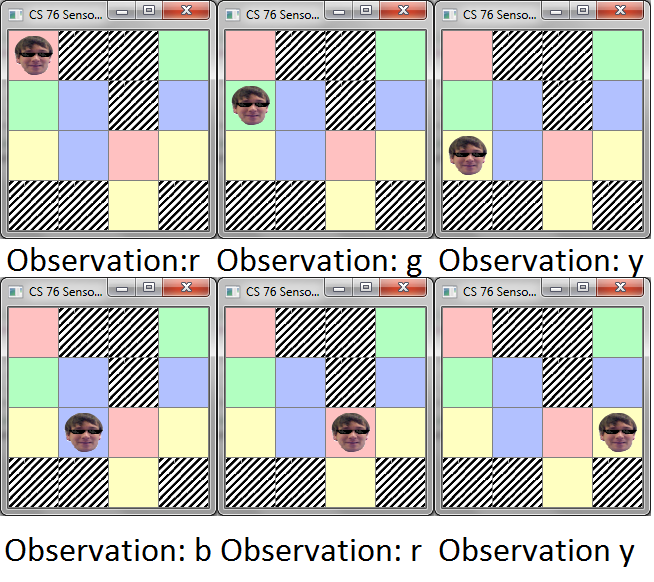
\includegraphics[width=1\textwidth]{4x4robotUnambiguous.png}
\caption{\label{fig:2x2 maze}path taken}
\end{figure}

\begin{figure}[H]
\centering
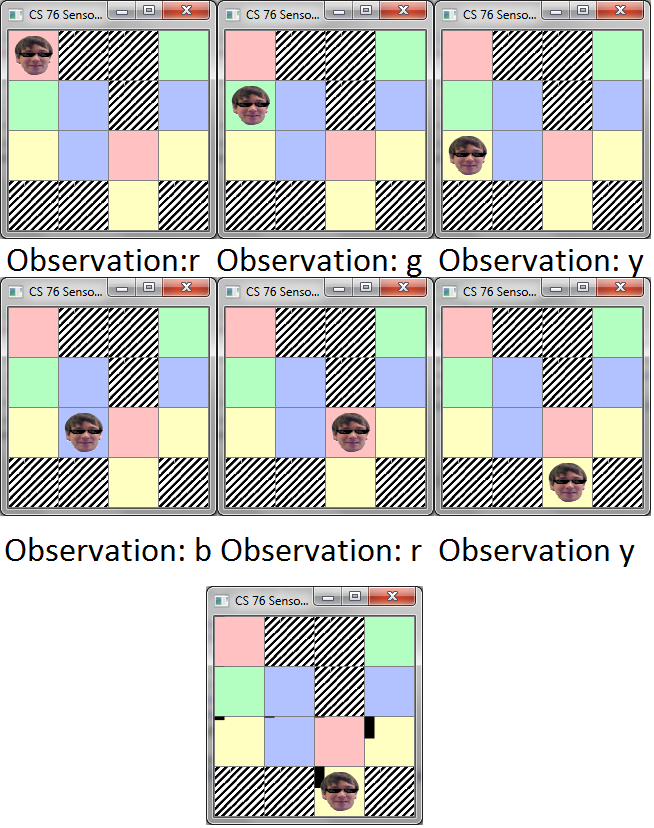
\includegraphics[width=1\textwidth]{4x4viterbiUnambiguous.png}
\caption{\label{fig:2x2 maze}viterbi path}
\end{figure}


Figures 17 and 18 show a similar phenomenon as figures 15 and 16. In this case, the robot finds it's way to the appropirate end tile, but on it's way instead of moving on an upward path along the red tiles, it starts and remains on the red tile between the two walls. 

\begin{figure}[H]
\centering
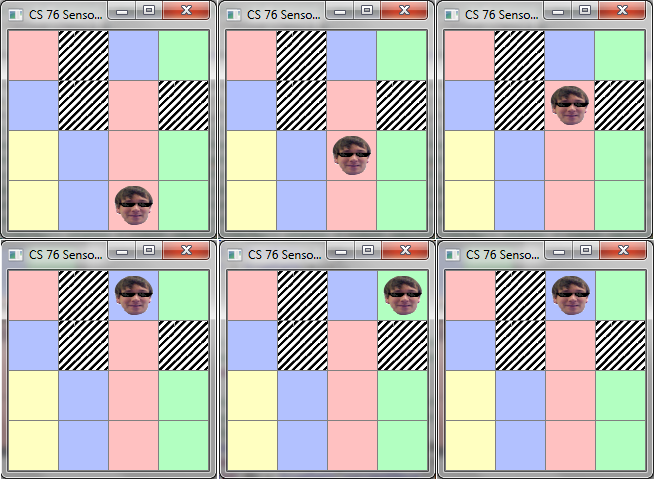
\includegraphics[width=1\textwidth]{viterbiPathwrongTruePath.png}
\caption{\label{fig:2x2 maze}path taken}
\end{figure}


\begin{figure}[H]
\centering
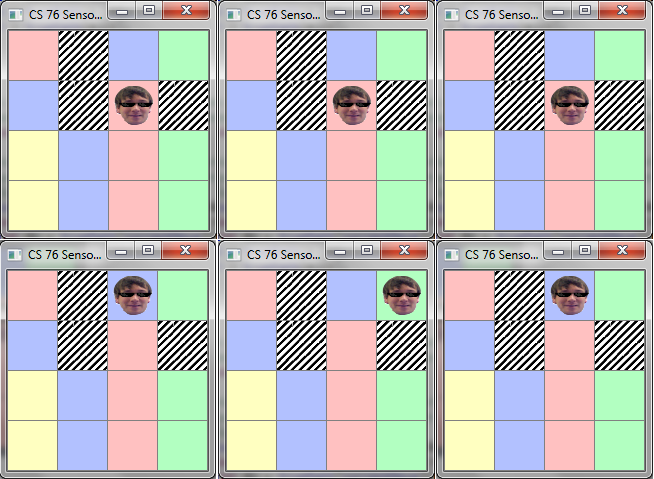
\includegraphics[width=1\textwidth]{viterbiPathwrong.png}
\caption{\label{fig:2x2 maze}viterbi path}
\end{figure}

The maze in figures 19 and 20 is very redundant. Each quadrant is identical. Viterbi has a particularly difficult time finding the actual path taken by the robot in redundant state spaces.

\begin{figure}[H]
\centering
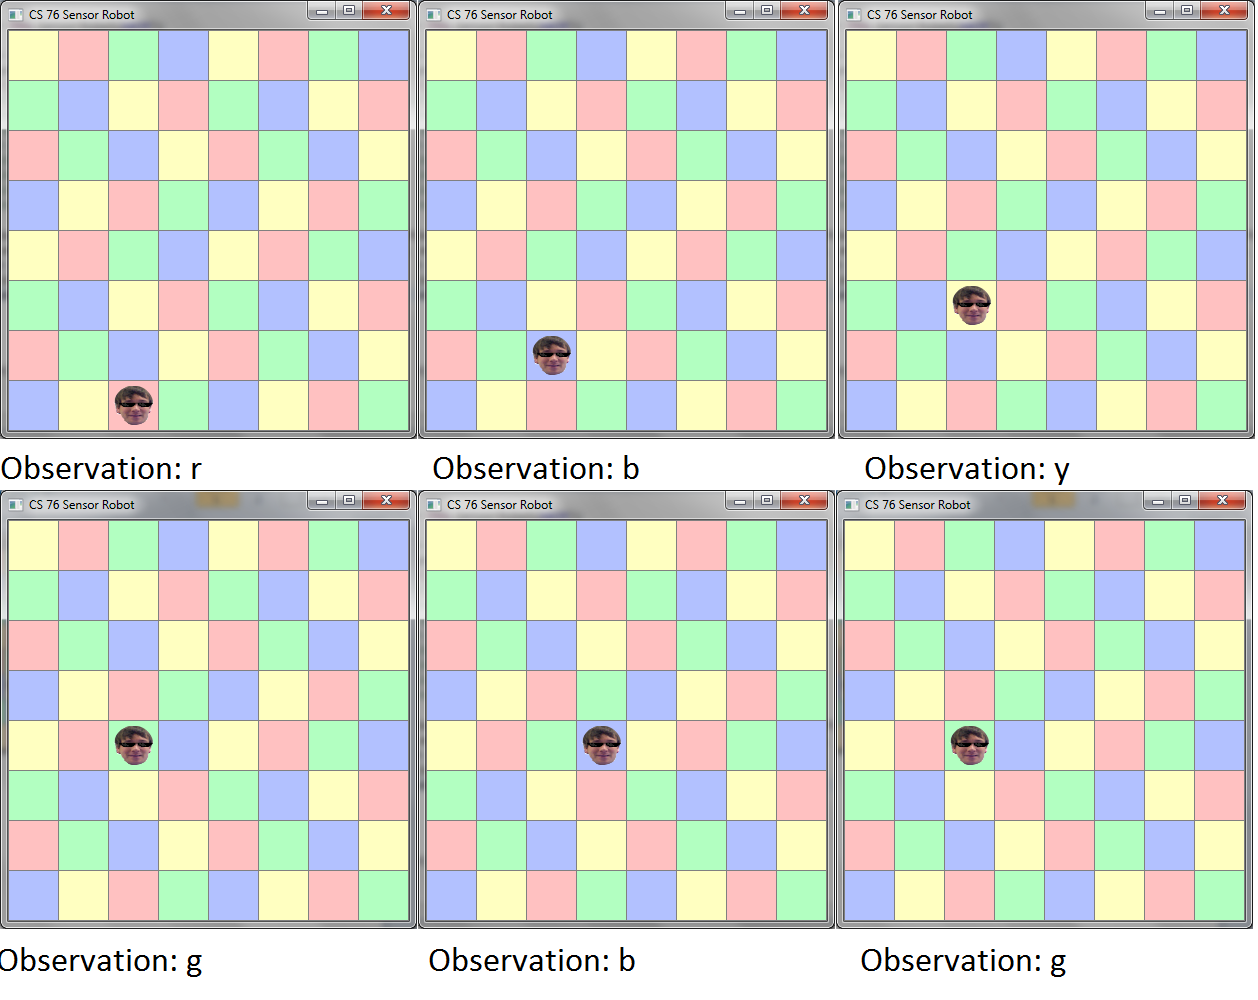
\includegraphics[width=1.2\textwidth]{10x10RobotAmbiguous.png}
\caption{\label{fig:2x2 maze}path taken}
\end{figure}

Note the probability distribution at time t. It is not concentrated on one tile. Rather it is spread accross all green tiles. All but one tile has a path to it which fits the observation sequence.

\begin{figure}[H]
\centering
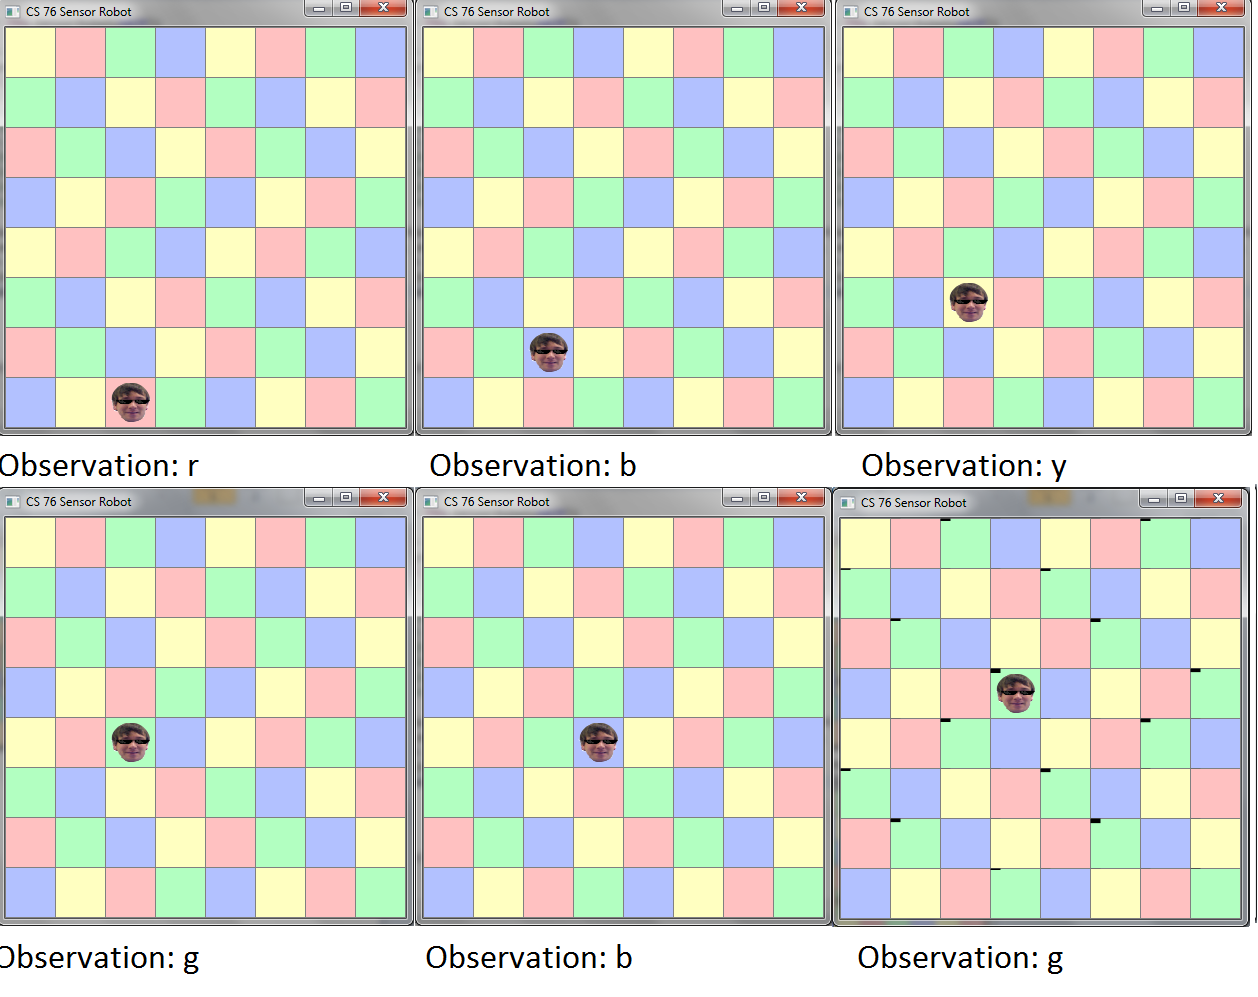
\includegraphics[width=1.2\textwidth]{10x10ViterbiAmbiguous.png}
\caption{\label{fig:2x2 maze}viterbi path}
\end{figure}

Figure 21 illustrates the number of paths through the maze. 

\begin{figure}[H]
\centering
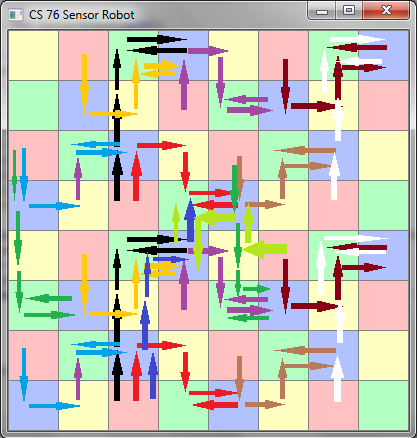
\includegraphics[width=1\textwidth]{Paths.png}
\caption{\label{fig:2x2 maze}vizualization of most paths in maze given the observations}
\end{figure}

\section{Conclusion}

Using HMMs, the robot was able to udate its belief state of location in the maze very efficiently, with good accuracy using filtering. When looking at past states, the robot was able to determine its location with great accuracy with some sacrifice of memory using the forward-backward algorithm. And it was able to find a path maximized over the probability of locations over time Viterbi. While prone to errors, using HMMs to infer the unobservable location of the robot in the maze was powerful given the low time complexities with respect to time.

\section{References}
Russell, Stuart J., and Peter Norvig. "Chapter 15 Probabilistic Reasoning Over Time." Artificial Intelligence: A Modern Approach. Upper Saddle River: Prentice-Hall, 2010. N. pag. Print.

\end{document}